\chapter{Example second chapter}
\label{chapter:second_ch}

This chapter is extensively based on the following publication:\\
\\
\fullcite{Aristeidou2024c}

\section{Introduction}

Example figures are shown in Figures \ref{sdof_bilinear_model} and \ref{Saavg3_FIV3_empirical_predicted_total_correlation}, inserted from a pdf file and svg file, respectively.

\begin{figure}
	\centering
	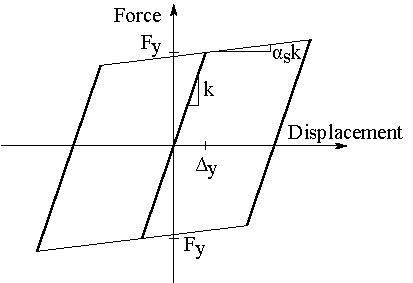
\includegraphics{figures_ch2/sdof_bilinear_model.pdf} % didn't specify width here
	\caption{Hysteretic behaviour of the bilinear \gls{SDOF} model (inserted from a pdf file)}
	\label{sdof_bilinear_model}
\end{figure}

\begin{figure}
	\centering
	\includesvg[width=1\textwidth]{figures_ch2/Saavg3_FIV3_empirical_predicted_total_correlation.svg}
	\caption{Empirical and corresponding predicted correlation coefficients between \gls{Saavg3} and \gls{FIV3} (inserted from an svg file)}
	\label{Saavg3_FIV3_empirical_predicted_total_correlation}
\end{figure}

\section{Discussion and conclusions}

This study presented the empirical correlations between assorted \glspl{IM} of various types, namely \gls{PGA}, \gls{PGV}, \gls{Sa}, \gls{Ds}, \gls{Saavg}, and \gls{FIV3}. The residuals, which are used for the calculation of correlations, were obtained from a previously developed \gls{GGMM} and the same filtered ground motion database. This is believed to produce more consistent correlation coefficients since the same database subset is used for the development of the \gls{GMM} and the calculation of empirical correlation coefficients.


